\documentclass[10pt, A4paper]{article}

\usepackage{amsmath}
\usepackage{amssymb}
\usepackage{amsthm}
\usepackage{mathtools}
\usepackage[linesnumbered,ruled]{algorithm2e}
\usepackage{booktabs}
\usepackage{graphicx}
\usepackage{subcaption}

\usepackage{natbib}
\setcitestyle{numbers, square}

\newtheorem{theorem}{Theorem}[section]
\newtheorem{lemma}[theorem]{Lemma}
\newtheorem{corollary}[theorem]{Corollary}

\newcommand{\mxm}{m \times m}
\newcommand{\mxn}{m \times n}
\newcommand{\nxn}{n \times n}
\DeclareMathOperator{\diag}{diag}
\DeclareMathOperator{\rank}{rank}

\newcommand*{\consoleFont}{\fontfamily{pcr}\selectfont}

%%%%%%%%%%%%%%%%%%%%%%%%%%%%%%%%%%%%%%%%%%%%%%%%%%%%%%%%%%%%%%%%%%%%%%

\begin{document}

\title{Polar Decomposition}
\author{Thomas Seleiro}
\maketitle


\begin{enumerate}
	\setcounter{enumi}{1}
	\item Prove that the singular values of $A$ are the eigenvalues of $H$.
\end{enumerate}

We know that any matrix $A\in\mathbb{C}^{\mxn}$, $m\geq n$ has 
a thin singular value decomposition $A = P \Sigma Q^*$ where $P \in
\mathbb{C}^{\mxn}$ has orthogonal columns, $Q \in 
\mathbb{C}^{\nxn}$ is unitary, and $\Sigma \in 
\mathbb{C}^{\nxn}$ is diagonal with $\Sigma = \diag(\sigma_1, 
\ldots, \sigma_r)$ where $\rank(A) = r$ and $\sigma_1 \geq \ldots \geq
\sigma_r \geq 0$, the singular values of $A$. Thus we can write
\begin{align}
	A = (PQ^*) (Q \Sigma Q^*) \eqqcolon UH
	\label{eq:PolarSVD}
\end{align}
where $U$ and $H$ satisfy the properties of a polar decomposition.

In particular we have $H = Q \Sigma Q^*$ where $\Sigma$ is diagonal and 
$Q$ is orthogonal. Thus the diagonal values of $\Sigma$ are the 
eigenvalues of $H$, which are the singular values of $A$.





\vspace{0.2cm}
\begin{enumerate}
	\setcounter{enumi}{2}
	\item Prove that $A$ is normal ($A^*A = AA^*$) iff $U$ and $H$
	commute.
\end{enumerate}

We first suppose that $U$ and $H$ commute. Note that for the product
$HU$ to be well defined, we must have $m = n$ which implies
$U\in\mathbb{C}$ is unitary. Since $A = UH = HU$ we get
\begin{align}
	\label{eq:AstarA}
	A^*A &= (UH)^* (UH) = H^*(U^*U)H = H^2 \\
	AA^* &= (HU) (HU)^* = H(UU^*)H^* = H^2
\end{align}
so $A$ is normal.

Now suppose $A$ is normal. Since $A^*A \in \mathbb{C}^{n\times n}$ and
$AA^* \in \mathbb{C}^{\mxm}$, $A$ normal requires $m=n$.
Using the singular value decomposition of $A$, we have
\begin{align}
	AA^* = (P\Sigma Q^*) (Q\Sigma P^*) = P\Sigma^2 P^*
	\label{eq:AAstar}
\end{align}
where $\Sigma^2 = \diag(\sigma_1^2, \ldots,\sigma_r^2)$.
Equating (\ref{eq:AstarA}) and (\ref{eq:AAstar}), we get 
$H^2 = P\Sigma^2P^*$. From~[\citealp{hojo1985}, p.405], we know 
that there
is a unique Hermitian positive semi-definite matrix $(AA^*)^{1/2}$ such 
that $(AA^*)^{1/2}(AA^*)^{1/2} = AA^* = H^2$.
It is obvious by its construction that $H$ is said matrix, but we also
note that $(P\Sigma P^*) (P\Sigma P^*) = P \Sigma^2P^* = AA^*$.
Therefore $H = P\Sigma P^*$ and
\begin{align}
	HU = (P\Sigma P^*) (PQ^*) = P \Sigma Q^* = A = UH
\end{align}
by the properties of the SVD of $A$. Therefore $U$ and $H$ commute.
 
 
 
 

\vspace{0.2cm}
\begin{enumerate}
	\setcounter{enumi}{3}
	\item Verify the formula
	\begin{align*}
		U = \frac{2}{\pi}A \int_{0}^{\infty} (t^2I - A^*A)^{-1}dt
		\tag{*}
		\label{eq:Q4}
	\end{align*}
	for full rank $A$ by using the singular value decomposition (SVD)
	of $A$ to diagonalize the formula.
\end{enumerate}

Since $A^*A = (Q\Sigma P^*)(P\Sigma Q^*) = Q\Sigma^2Q^*$, we have
\begin{align}
	t^2I + A^*A = Q(t^2I)Q^* + Q \Sigma^2Q^* = QDQ^*
	\label{eq:Q4eq1}
\end{align}
where $D \coloneqq \diag(t^2 + \sigma_i)$.
Inverting (\ref{eq:Q4eq1}) gives
\begin{align}
	(t^2I + A^*A)^{-1} = QD^{-1}Q^*, \qquad
	D^{-1} = \diag\left(\frac{1}{\sigma_i^2 + t^2} \right)
\end{align}
Since $Q$ and $Q^*$ do not depend on $t$, they can be taken outside the 
integral, leaving the right hand side of~(\ref{eq:Q4}) in the form
\begin{align}
	\frac{2}{\pi} A\, Q\int_{0}^{\infty}D^{-1}dt\, Q^*.
\end{align}
The integral is a diagonal matrix where the $i$th diagonal component is
\begin{align}
	\int_{0}^{\infty} \frac{1}{\sigma_i^2 + t^2} \, dt =
	\left[\frac{1}{\sigma_i} \arctan \left(\frac{t}{\sigma_i}\right)
	\right]_0^{\infty} = \frac{\pi}{2\sigma_i}
\end{align}
using~[\citealp{jeda2008}, 4.2.4.4]. So the right-hand side of 
(\ref{eq:Q4}) is
\begin{align}
	\begin{split}
	A\,Q\diag\left(\sigma_i^{-1}\right)Q^*&=
	P\Sigma Q^* \, Q \Sigma^{-1}Q^* = PQ^* = U 
%	\Sigma^{-1} isn't necessarily well defined
	\end{split}
\end{align}





\vspace{0.2cm}
\begin{enumerate}
	\setcounter{enumi}{4}
	\item Derive Newton's method for computing U by considering
	equations $(X+E)*(X+E) = I$, where $E$ is a ``small perturbation''.
	(Newton's method is $X_{k+1} = (X_k + X_k^{-*})/2, X_0 = A$)
\end{enumerate}

We know that $U$ is the closest unitary matrix to $A$, and since 
$U^*U=I$, we try to find a solution to the equation
\begin{align}
	F(X) = 0,\qquad F(X)\coloneqq X^*X - I
\end{align}
using a Newton method starting at $A$.
The general form of the Newton method [\cite{Kell2003}, p.] is
\begin{align}
	F(X_{k+1}) + DF_{X_k} \left[X_{k+1} - X_k\right] = 0
	\label{eq:genNewt}
\end{align}
where $DF_{X_k}$ is the Fréchet derivative and, is the first order $E$ 
term in
\begin{align}
	F(X+E) - F(X) = X^*E + E^*X + E^*E.
\end{align}
So $DF_{X_k}[E] = X^*E + E^*X$. Substituting in~(\ref{eq:genNewt}),
\begin{align}
	X_k^*X_k - I + X_k^* \left( X_{k+1} - X_k \right) + 
		\left( X_{k+1}^* - X_k^* \right)X_k &= 0 \\
	X_k^*X_k - I + X_k^* X_{k+1} - X_k^* X_k + 
		X_{k+1}^* X_k - X_k^*  X_k &= 0 \\
	X_k^* X_{k+1} + X_{k+1}^*X_k &= X_k^* X_k + I
\end{align}
We know that for any matrix we can write $B = 1/2(B + B^*) + 
1/2(B-B^*)$, where the terms on the right-hand side are the Hermitian 
and skew Hermitian components respectively [\citealp{hojo1985}, p.170].
Setting the skew Hermitian part to zero, and taking $B = X_k^*X_{k+1}$ 
gives
\begin{align}
	X_k^*X_{k+1} &= \frac{1}{2} \, (X_k^*X_k + I) \\
	X_{k+1} &= \frac{1}{2} \, (X_k + X_k^{-*})
	\label{eq:newton}
\end{align}





\vspace{0.2cm}
\begin{enumerate}
	\setcounter{enumi}{5}
	\item Prove that Newton's method converges, and at a quadratic
	rate, by using the SVD of $A$.
\end{enumerate}

For the Newton iteration to be well defined, we require that $A$ and 
the iterates $X_k$ be invertible.

We have the SVD of $A = P\Sigma Q^*$ and $U = PQ^*$.
The iterates $X_k$ also have a singular value decomposition, which we 
write $X_k=P_k \Sigma_k Q_k^*$. Using this in eq.~(\ref{eq:newton}) 
gives
\begin{align}
	X_{k+1} = (X_k + X_k^{-*})/2 &= \frac{1}{2} (P_k \Sigma_k Q_k^* + 
	P_k \Sigma_k^{-1} Q_k^*)\\
	&= P_k \frac{1}{2}(\Sigma_k + \Sigma_k^{-1}) Q_k^*
\end{align}
So we can identify the factors in the SVD of $X_{k+1}$ (up to 
reordering of rows) and get 
\begin{align}
	P_k = P, \qquad Q_k = Q, \qquad \Sigma_{k+1} = \frac{1}{2}
	\left(\Sigma_k + \Sigma_k^{-1} \right)
\end{align}

We now have
\begin{align}
	U - X_{k+1} &= PQ^* - P\left[\frac{1}{2}
	\left(\Sigma_k + \Sigma_k^{-1}\right)\right] Q^* \\
	&= \frac{1}{2} P \left[\left(I - \Sigma_k\right) + 
	\left(I - \Sigma_k^{-1}\right) \right] Q^* \\
\end{align}
And since
\begin{align}
	- \Sigma_k^{-1} (I - \Sigma_k)^2 &= -\Sigma_k^{-1}
	\left(I - 2 \Sigma_k + \Sigma_k^2\right) \\
	&= 2I -\Sigma_k - \Sigma_k^{-1}
\end{align}
we are left with $U - X_{k+1} = -P \Sigma_k^{-1} \left( I - \Sigma_k
\right)^2 Q^* /2$.
Taking the 2-norm on both sides and exploiting the fact that $P$ and 
$Q$ are orthogonal,
\begin{align}
	\| U - X_{k+1} \|_2 &\leq \frac{1}{2}\, \left\| P\Sigma_k^{-1} 
	\right\|_2 \left\| (I - \Sigma_k)^2 Q^*\right\|_2 \\
	&= \frac{1}{2}\, \left\|\Sigma_k^{-1}\right\|_2 \left\| \left( I - 
	\Sigma_k \right)^2 \right\|_2 \\
	&\leq \frac{1}{2}\, \|X_k\|_2 \|I - \Sigma_k\|_2^2 \\
	&= \frac{1}{2}\, \|X_k\|_2 \|U - X_k\|_2^2
\end{align}

To achieve quadratic convergence, we need to bound $\|X_k\|$ by a 
constant. We do so by observing that
\begin{align}
	\|X_{k+1}\|_2 = \max_{i = 1:n} \frac{\sigma_i + \sigma_i^{-1}}{2}
	\leq \max \left\{ \left\|X_k \right\|_2
	, \left\|X_k^{-1} \right\|_2 \right\}
\end{align}
and so for all $k$, $\|X_k\|_2 \leq M \coloneqq \max\{\|A\|_2, 
\|A^{-1}\|_2\}$.
Thus we conclude that the Newton method converges quadratically.





\vspace{0.2cm}
\begin{enumerate}
	\setcounter{enumi}{6}
	\item Use the SVD to analyse the convergence of the
	Newton\nobreakdash-Schulz iteration for computing $U$:
	\begin{align*}
		X_{k+1} = \frac{1}{2}X_k(3I - X_k^* X_k), \qquad X_0 = A
	\end{align*}
\end{enumerate}

We assume $A \in \mathbb{C}^{\mxn}$ and $m\geq n$. We replace $A$ in 
the expression of $X_1$ with the thin SVD $A = P \Sigma Q^*$ and get
\begin{align}
	X_1 = \frac{1}{2}P \Sigma Q^*(3I - Q\Sigma P^* P \Sigma Q^*)
	   &= \frac{1}{2} P \Sigma (Q^* Q) (3I - \Sigma^2) Q^* \\
	   &= P \left[ \frac{1}{2} (3\Sigma - \Sigma^3) \right] Q^*.
\end{align}
Thus we can write $X_1 = P \Sigma_1 Q^*$ where $\Sigma_1 = (3\Sigma - 
\Sigma^3)/2$.
Applying the same method recursively we can write $X_k = P\Sigma_k Q^*$ 
with
\begin{align}
\Sigma_k = \diag(\sigma_i^{(k)}), \qquad \Sigma_{k+1} = \diag
(3\sigma_i^{(k)} - (\sigma_i^{(k)})^3).
\end{align}
In order for the method to converge, we require every diagonal element 
of $(\Sigma_k)_{k\in\mathbb{N}}$ to converge. Since we want $X_k$ to 
converge to $U = PQ^*$, we want each diagonal element to converge to 1. 

We consider the real sequence $(x_k)_{k \in \mathbb{N}}$ defined by the 
recurrence relation
\begin{align}
	x_{k+1} = p(x_k), \qquad x_0 \geq 0, \qquad p(x) \coloneqq 
	\frac{1}{2} (3x - x^3),
\end{align}
where the condition $x_0 \geq 0$ is motivated by the singular values of 
$A$.

We first note that $p$ is an odd function with roots at 0, $\pm\sqrt{3}$
and local maxima at $\pm1$ ($p(\pm1) = \pm1$).
Since the leading coefficient of $p$ is negative, $p$ is positive on 
$[0,\sqrt{3}]$ and negative on $[\sqrt{3}, \infty)$. We now study the 
convergence of $(x_k)$ for different values of $x_0$.
\begin{itemize}
	\item For $x_0 = 0$ or $\sqrt{3}$, $x_0$ is a root of $p$ so $x_k 
	\to 0$ as $k \to \infty$.
	\item For $0 < x_0 \leq 1$, $p(0,1) = (0, 1)$ and $p(x) > x$  on 
	$(0, 1)$ so $x_k \to 1$ as $k \to \infty$.
	\item For $1 < x_0 < \sqrt{3}$, $p(x_0) \in (0,1)$ so $x_n = 
	p^n(x_0) = p^{n-1}(p(x_0)) \to 1$ as $k \to \infty$.
	\item For $x_0 > \sqrt{3}$, $p(x_0)$ is negative so we cannot 
	guarantee convergence to 1. It is easy to show that for $x_0 \geq 
	\sqrt{5}$ the iteration diverges, since $|p(x)| \geq x$ and $p$ is 
	unbounded for $|x| \geq \sqrt{5}$.
\end{itemize}
Therefore, every diagonal sequence converges to 1 if $0 < \sigma_i < 
\sqrt{3}$ for $i = 1:\rank(A)$, or equivalently $\|A\|_2 < \sqrt{3}$ 
and $A$ is full rank.

It follows that for a starting matrix $A$ with full rank and $\|A\|_2 < 
\sqrt{3}$,
\begin{align}
	\|U-X_{k+1}\|_2 &= \left\|PQ^* - P\left[\frac{1}{2}(3 \Sigma_k
	-\Sigma_k^3)\right] Q^*\right\|_2
	= \left\|I - \frac{1}{2}(3\Sigma_k - \Sigma_k^3)\right\|_2 \\
	&= \max_{i = 1:n} \left|1 - \frac{1}{2}\left(3 \sigma_i^{(k)} - 
	(\sigma_i^{(k)})^3\right)\right|,
\end{align}
which tends to 0 as $k \to \infty$.





\vspace{0.2cm}
\begin{enumerate}
	\setcounter{enumi}{7}
	\item Evaluate the operation count for one step of Newton's 
	method and one step of the Newton\nobreakdash-Schulz iteration (taking
	account of symmetry). Ignoring operation counts, how much faster
	does matrix multiplication have to be than matrix inversion for
	Newton\nobreakdash-Schulz to be faster than Newton (assuming both take the same number of iterations)?
\end{enumerate}

We first consider the $k$th step $X_{k+1} = (X_k + X_k^{-*})/2\,$ for 
the Newton iteration of a matrix $A \in \mathbb{C}^{n\times n}$. We 
identify 3 main operations:
\begin{itemize}
	\item One matrix inversion of $X_k \in \mathbb{C}^{\nxn}$: 
	\hfill
	$2n^3 + O(n^2)$ flops
	
	\item One matrix addition in $\mathbb{C}^{\nxn}$:
	\hfill
	$n^2$ flops
	
	\item One element-wise division in $\mathbb{C}^{\nxn}$:
	\hfill
	$n^2$ flops
\end{itemize}
So the total number of operations for the Newton method is $2n^3 + 
O(n^2)$.

We now consider a step of the Newton-Schulz iteration $X_k(3I - 
X_k^*X_K)/2$ for $X_0 = A \in \mathbb{C}^{\mxn}$.
We fist note that $X_k^*X_k$, and by extension $(3I - X_K^*X_k)/2$, is 
Hermitian in $\mathbb{C}^{\nxn}$.
Therefore only the upper triangular elements of these matrices need to 
be calculated, ie we only have to compute $\sum_{k=1}^{n} k= (n^2+n)/2$ 
components.
Calculating $X_k*X_k$, we use the Algorithm~\ref{alg:XstarX},
\begin{algorithm}
	$b_{ij} = (X_k^*X_k)_{ij}$ \;
	\For{$i = 1:n$}
	{
		\For{$j = i:n$}
		{
			\For{$r = 1:m$}
				{
					$b_{ij} = b_{ij} + \overline{x_{ri}}x_{rj}$ \;
				}
		}
	}
	\caption{Algorithm to compute the top diagonal elements of 
	$X_k^*X_k$}
	\label{alg:XstarX}
\end{algorithm}
using a total of $mn^2 + mn$ flops. Forming $3I - X_k^*X_k$ and 
dividing the result by 2 adds $n^2 + n$ operations. Finally multiplying 
by $X_k$ takes $2mn^2$ flops for a total of $3mn^2 + O(n^2) + O(mn)$ 
flops per step.







\vspace{0.2cm}
\begin{enumerate}
	\setcounter{enumi}{8}
	\item Write a MATLAB M-file \texttt{poldec} that computes the 
	polar decomposition of a nonsingular $A \in \mathbb{C}^{\nxn}$.
\end{enumerate}

We wrote the MATLAB function \texttt{poldec} (see \texttt{poldec.m} in 
the github repository 
\emph{https://github.com/ThomasSeleiro/PolarDecompProj})
that computes the polar decomposition of a matrix $A$.

The two variables \texttt{newtSchulz} and \texttt{converged} control 
the function's operation.
The function starts by computing $U$ using the Newton's method, until
the condition $\|X_k\|_2 < \sqrt{3}$ stored in \texttt{newtSchulz} 
turns true. 
From this point onwards, the function begins 
using the {Newton-Schulz} iteration to calculate $U$.

The function stops iterating once the variable
\begin{verbatim}
	converged = (unitDist <= 1e-16) || (iterDist <= 1e-16);
\end{verbatim}
becomes true.
Here \texttt{unitDist} stores the value $\|I -X_k^*X_k\|_\infty$ and 
\texttt{iterDist} stores $\|X_k - X_{k-1} \|_\infty / \|X_k\|_\infty$.
We motivate this choice for convergence by noting that if either 
distance is of the order of the unit roundoff $u = 10^{-16}$, the 
iterates stop gaining precision in double floating point arithmetic.
For example, if \texttt{unitDist} $< u$, the matrix $X_k$ is unitary to 
machine precision. Similarly, if \texttt{iterDist} $< u$, the iterates 
$X_k$ and $X_{k-1}$ are sufficiently close in double precision floating 
point arithmetic, and any subsequent iterates will be close to $X_k$.
Note that a maximum number of 1000 iterates per computation was set to 
avoid long computation times if the algorithm doesn't manage to reduce 
\texttt{unitDist} or \texttt{iterDist} enough.

Once $U$ is calculated, we simply form $H = U^*A$ to output the full 
polar decomposition.



\begin{figure}[t]
	\centering
	\begin{subfigure}{0.5\textwidth}
		\centering
		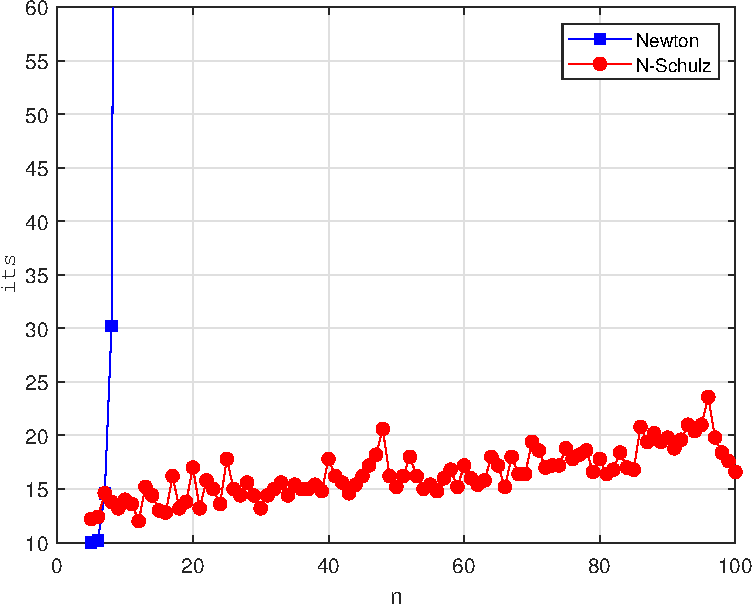
\includegraphics[width=.8\linewidth]{randnIts.pdf}
		\caption{\label{fig:randnIts}}
	\end{subfigure}%
	\begin{subfigure}{0.5\textwidth}
		\centering
		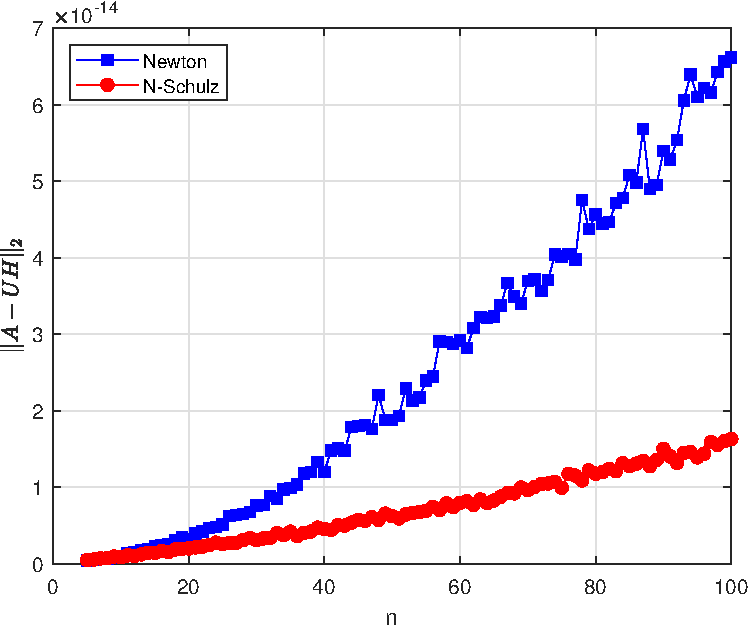
\includegraphics[width=.8\linewidth]{randnAccuracy.pdf}
		\caption{\label{fig:randnAccuracy}}
	\end{subfigure}
	\caption{
	Figure showing (a) the number of iterations and 
	(b) the accuracy of the polar decomposition of 
	\texttt{rand(n)} computed using the Newton method only, and the 
	\texttt{poldec} function. Note in (a) that the Newton only method 
	quickly reaches the maximum allowed number of iterations at $n = 
	11$.
	\label{fig:randn}}
\end{figure}
We first tested the implementation of \texttt{poldec} by using random 
matrices of size $n$ using the MATLAB function \texttt{rand(n)}. The 
results of these experiments are summarised in Fig.~\ref{fig:randn}.
We note that \texttt{poldec} which uses the Newton-Schulz iteration 
converges significantly quicker and produces a more accurate result.
Quicker convergence for the Newton method could be achieved by using 
more lenient convergence criteria, but this would likely lead 
to decreased accuracy of the computed decomposition. 

\begin{table*}[h]
	\centering
	\begin{tabular}{ l c c c c c }
		\toprule
		& & \multicolumn{2}{c}{\texttt{its}} & 
		\multicolumn{2}{c}{$\|A-UH\|_2$} \\
		\cmidrule(lr){3-4} \cmidrule(lr{12pt}){5-6}
		$A$ & $\kappa_2(A)$ & Newton only & \texttt{poldec} & Newton only 
		& 
		\texttt{poldec} \\
		\midrule
		\texttt{eye(8)} & 1 & 1 & 1 & 0 & 0 \\
		\texttt{hilb(6)} & 1.5e07 & 28 & 31 & 0 & 1.9230e-16 \\
		\texttt{magic(6)} & 4.7e16 & 68 & 60 & 1.8465e-14 & 
		1.4991e-14 \\
		\texttt{hadamard(8)} & 1 & 124 & 12 & 8.1113e-16 & 7.0890e-16\\
		\bottomrule
	\end{tabular}
	\caption{
	Results of experiments applying \texttt{poldec} 
	to	various matrices. A variant of the function that only uses the 
	Newton method was also used for comparison. Results obtained by 
	running \texttt{otherTest.m}
	\label{tab:poldecresults}}
\end{table*}

Table~\ref{tab:poldecresults} shows metrics related to computing the 
polar decomposition of a few specific matrices using \texttt{poldec} 
and a function using only the Newton method.

We see that only one iteration is needed for the identity matrix 
\texttt{eye(8)} since it is already unitary.

Using \texttt{hilb(6)} as input illustrates the case when A is hermitian 
positive definite.
It is clear in this case that $U = I$ since $H$ is a hermitian positive 
definite matrix.
However, both algorithms take a long time to compute $U$ since they are 
unable to make these deductions. Since $U= I$ however, the 
result is accurate to machine precision.

The function takes a relatively large number of iterations to find the 
polar decomposition of \texttt{magic(6)}. We note that for any matrix $A$,
$$M \coloneqq \max \left\{\|A\|_2, \|A^{-1}\|_2 \right\} \geq 
\kappa_2(A)^{1/2}.$$
Since for the Newton method
$$\|U - X_{k+1}\|_2 \leq \frac{M}{2} \|U - X_k\|_2^2,$$
for large values of $M$ convergence will be slow.
This explains the larger number of iterations for both \texttt{hilb(6)} 
and \texttt{magic(6)}.

For the computation of the polar decomposition of \texttt{hadamard(8)}, 
we achieve good accuracy and a small number of iterations using the 
\texttt{poldec} function. For the Newton method only, while the 
iterations did not achieve the convergence criterion, both 
\texttt{iterDist} and \texttt{unitDist} rapidly decrease past 
$10^{-15}$ but keep fluctuating for a long time before one eventually 
drops below $10^{-16}$. The output of the Newton only script is shown 
below.
\begin{verbatim}
k   	 |X_k-X_{k-1}|/|X_k|   |I - X_k^*X_k|
=== 	    ==============     ==============
                    [...]
5	       1.46536674e-05	    2.14730583e-10
6	       1.07365042e-10	    9.33334681e-16
7	       4.31775426e-16	    1.54939455e-15
8	       5.49532361e-16	    1.51620177e-15
                    [...]
121	     2.35513869e-16	    6.09764714e-16
122	     2.15887713e-16	    6.08974934e-16
123      1.17756934e-16	    5.84808662e-16
124      7.85046229e-17	    5.59620674e-16
\end{verbatim}

We also compared the runtime of \texttt{poldec} and a simple Newton's 
method over the same number of iterates (taken from the number of 
iterates required for the Newton only iteration to converge).
\begin{table*}[t]
	\centering
	\begin{tabular}{ l c c c }
		\toprule
		& &\multicolumn{2}{c}{Runtime (in ms)} \\
		\cmidrule(lr){3-4}
		$A$ & \texttt{its} & Newton only & \texttt{poldec} \\
		\midrule
		\texttt{rand(8)}     & 12   & 1.574  & 1.166  \\
		\texttt{rand(20)}    & 1000 & 78.362 & 52.129 \\
		\texttt{hilb(6)}     & 28   & 1.513  & 1.608  \\
		\texttt{magic(6)}    & 68   & 7.951  & 3.248  \\
		\texttt{hadamard(8)} & 124  & 10.857 & 4.799  \\
		\bottomrule
	\end{tabular}
	\caption{
	Runtimes when calculating the Polar Decomposition using 
	Newton's method and the function \texttt{poldec}. Results obtained 
	by running \texttt{speedTest.m}
	\label{tab:runtimes}}
\end{table*}
Table~\ref{tab:runtimes} shows the times taken to compute the polar 
decompositions of some of the matrices. Overall the computation time 
remains lower in most cases for the \texttt{poldec} function.
This suggests that thanks the matrix multiplication implementation is 
much faster than matrix inversion, as mentioned in Question 8.





\vspace{0.2cm}
\begin{enumerate}
	\setcounter{enumi}{9}
	\item Write another routine that computes the square root of a 
	Hermitian positive definite matrix by doing a Cholesky 
	decomposition and calling \texttt{poldec}.
\end{enumerate}

For any Hermitian positive definite matrix $A \in \mathbb{C}^{\nxn}$, 
we can compute the unique Cholesky factorization $A = R^*R$, where $R 
\in \mathbb{C}^{\nxn}$ is an upper-triangular matrix with strictly 
positive diagonal values.
Since the Cholesky factor is full rank, we can compute its polar 
decomposition $R = UH$ with $U$ unitary and $H$ hermitian positive 
definite.
Using this decomposition, we get $$A = R^*R = (UH)^*UH = H^2.$$
Hence $H$ is the matrix square root of $A$.

We implemented the discussed method for calculating square roots in the 
function \texttt{poldecsqrt} (in the \texttt{.m} file of the same name).
We used the MATLAB function \texttt{chol} to calculate the Cholesky 
factor \texttt{R} of the input matrix \texttt{A}.
\texttt{poldec} is then used to find the Hermitian factor \texttt{H} of 
\texttt{R}. Note the function raises an error if the input matrix is 
not Hermitian positive definite.


\bibliography{mybib}
\bibliographystyle{plain}


\end{document}